\section{Descripción del lugar de ejecución}
La Región Puno tiene una historia grandiosa de origen, de culturas pre-incas: Pukara, Tiahuanaco, Lupaca entre otros, Inca, cuyas manifestaciones aún se mantienen vivas, muchas ubicadas alrededor del Lago Titicaca, contamos con productos como la quinua, papa, alpaca entre otros, que son un aporte a la humanidad, los majestuosos paisajes que ofrece el Lago Titicaca hasta las magníficas vistas de Macusani, Carabaya, con arte rupestre y aguas termales, y la inmensa biodiversidad de la selva Puneña; La arquitectura colonial manifestada en Templos, casonas, balcones que datan del siglo XVI en Lampa, Juli, Puno, atractivos que hacen que la región tenga un potencial turístico de nivel internacional \cite{2011PlanPERTUR}. Puno es la cuarta ciudad más visitada por extranjeros, a nivel nacional, después de Lima y Callao, Cusco y Arequipa. \cite{2016CarpetaPeru}.

\subsection{Ubicación geográfica}
La región Puno está ubicado al extremo sur este del Perú, el territorio comprende 61,0\% de sierra, un 32,1\% de zona de selva, 0,02\% de superficie insular(islas) y 6,9\% que corresponden a la parte peruana del Lago Titicaca (considerado el lago navegable más alto del mundo, a 3,827 m.s.n.m.) \cite{2016CarpetaPeru}.

Según \citeA{2011PlanPERTUR} Puno tiene una ubicación geopolítica estratégica en el continente, y una ubicación estratégica en el corredor turístico Cusco - Puno - La paz (Bolivia); con Cusco como la gran atracción turística con el Santuario de Machu Picchu (maravilla cultural del mundo moderno), así como con las regiones de Arequipa y Tacna, esta última con gran afluencia de turistas chilenos. Y la carretera interoceánica sur que conecta a la Región de Puno a través de Madre de Dios con Brasil, lo que permite la afluencia de turistas brasileros.

\subsection{Clima}
El clima en general de la región de Puno varía entre frío y cálido. Por su localización geográfica, su altitud y proximidad al Lago Titicaca que tiene efecto termorregulador. La temperatura promedio anual de 8.7°C, con estaciones marcadamente secas y húmedas, las temperaturas máximas y mínimas en el día, presentan fuertes oscilaciones propias del altiplano, entre los 13.3°C (junio y julio) a 16.1° (noviembre) y -1.0°C (junio), siendo el clima frío en cualquier época del año. El clima no es problema para el desarrollo del turismo, lo que causa ciertos estragos es la altura sobre el nivel del mar, que a veces cuando no se toman adecuadas precauciones, causa malestares en la persona, como el mal de altura (soroche). Las precipitaciones pluviales en el altiplano, obedecen a una periodicidad anual de cuatro meses (diciembre a marzo); esta periodicidad, a pesar de determinar las campañas agrícolas, puede variar según las características pluviales del año, originando inundaciones o sequías, así como la presencia de heladas y granizadas. \cite{2011PlanPERTUR,2016CarpetaPeru}.

\subsection{Accesibilidad en la región}
“En la región de Puno, existen cuatro medios de transporte, según su importancia son transporte terrestre, aéreo, férreo y lacustre. Cuenta con una red vial que permite la conexión con las regiones de la macro región sur, y de la capital de la región con las capitales provinciales, vías con diferentes condiciones, asfaltadas, afirmadas y trochas carrozables que, de acuerdo a la ubicación de los atractivos, influyen en los flujos turísticos.” \cite{2011PlanPERTUR}

\subsubsection{Accesibilidad terrestre}
Esta conformado por los siguientes ejes viales según \citeA{2011PlanPERTUR}, como se puede observar también en la figura \ref{fig:mapa_vial_puno}:
\begin{itemize}
    \item CUSCO - La Raya, Ayaviri, Juliaca, Puno
    \item BOLIVIA - Desaguadero - Yunguyo, Juli, Ilave, Puno
    \item AREQUIPA - Lagunillas, Santa Lucía, Juliaca
    \item MADRE DE DIOS - Puente Inambari, San Gaban, Ollachea, Macusani, Azangaro, Juliaca
    \item TACNA - Capazo, Mazocruz, Conduriri, Ilave
    \item MOQUEGUA - Titiri, Laraqueri, Puno
    \item MOQUEGUA - Santa Rosa, Mazocruz, Huacullani, Desaguadero
    \item BOLIVIA - Tilaly, Conima, Moho, Huancane, Juliaca
    % Estan sin considerar las locale(provinciales)
\end{itemize}
\begin{figure}[!ht]
    \centering
    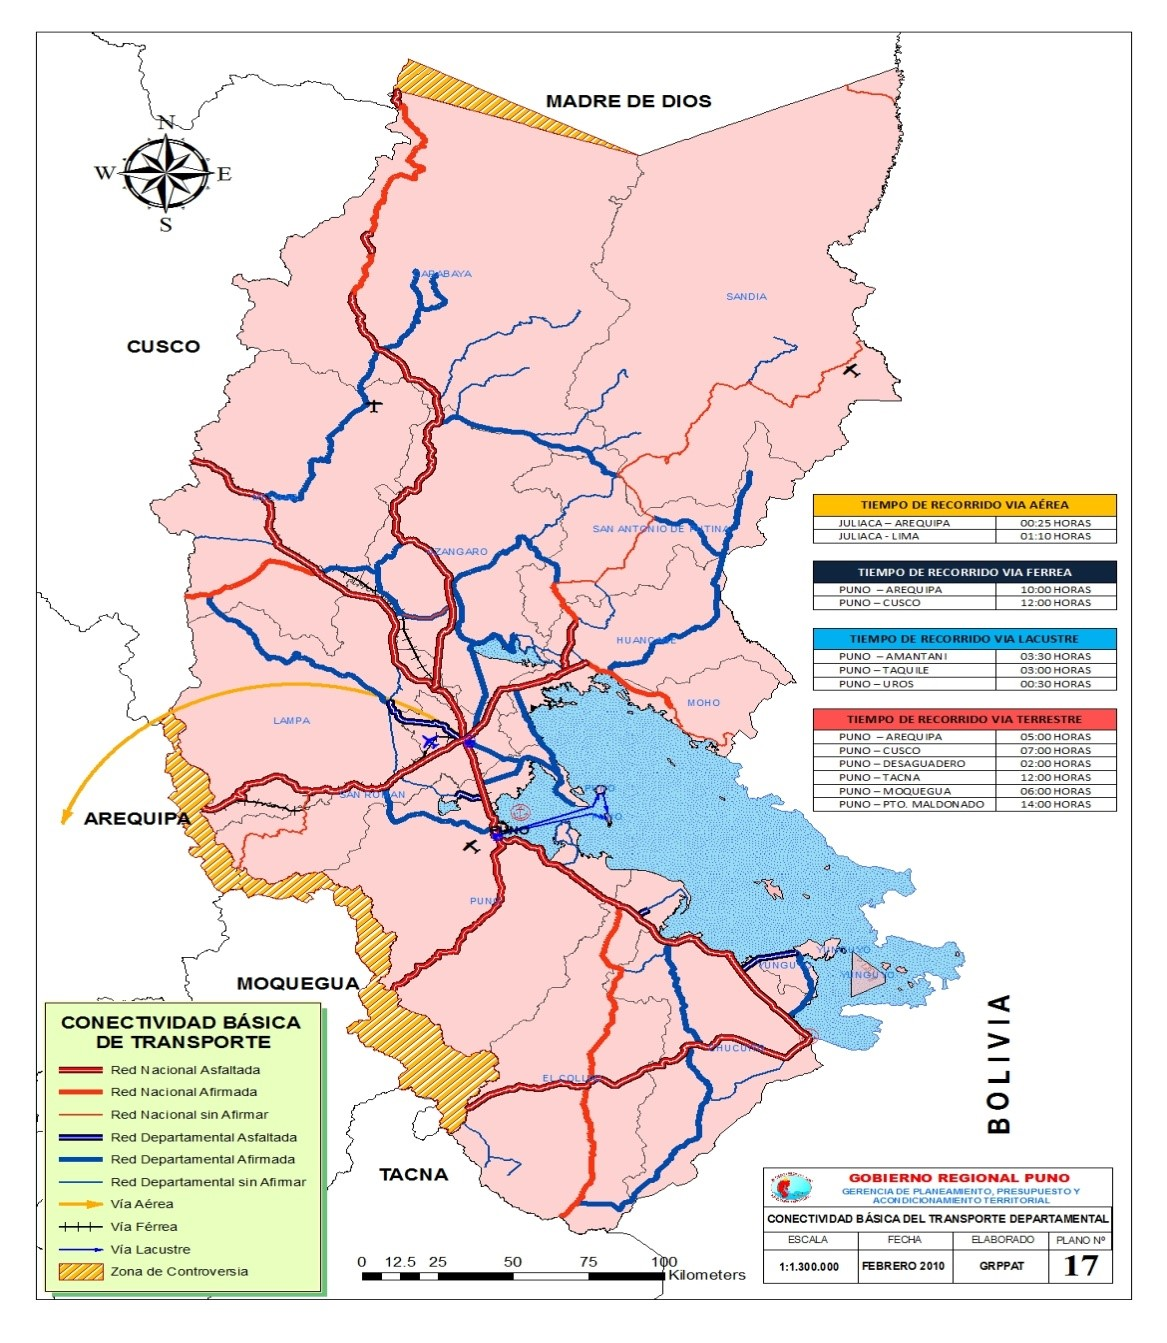
\includegraphics[scale=1]{Capitulo4/Figs/mapa-vial-puno.jpg}
    \caption{Mapa vial de la región Puno}
    Fuente: \citeA{2011PlanPERTUR}
    \label{fig:mapa_vial_puno}
\end{figure}

\subsubsection{Accesibilidad aérea}
Existen dos lineas aéreas que hacen el servicio de pasajeros y carga desde Lima; Lan Perú, y Star Perú, y a través de las principales ciudades de la macro región; Cusco, Arequipa y Tacna, hasta y desde la ciudad de Juliaca. En la región existen dos pistas de aterrizaje autorizadas; El aeropuerto Inca Manco Capac de la Ciudad de Juliaca(en el cual se desplazan los turistas en su visita a la región de Puno), y el aeródromo de la Compañía minera MINSUR – Mina San Rafael ubicado en el distrito de Antauta de la Provincia de Melgar(no se realizan vuelos de carácter comercial) \cite{2011PlanPERTUR}.

\subsubsection{Accesibilidad férrea}
El ferrocarril del sur del Perú, conecta Puno con Arequipa y Cusco, en los últimos años ha decaído su importancia, aunque continúa operando y brindando servicios de carga y pasajeros, moviliza el 17.54\% de pasajeros y 14.68\% de los volúmenes de carga. La empresa Perú Rail ha privilegiado atender el transporte turístico de pasajeros en la ruta Puno - Juliaca - Cusco - Machu Picchu, con frecuencia diaria a las 8:00 am.. Solo se transporta carga entre las ciudades de Puno Arequipa. La longitud ferroviaria del sur alcanza a 992 kms, une Puno, Juliaca, Arequipa y Matarani, Cusco y Quillabamba \cite{2011PlanPERTUR}.

\subsubsection{Accesibilidad lacustre}
Por este medio se moviliza aproximadamente el 3.94\% de pasajeros de la región, el transporte de carga se circunscribe al traslado de productos de primera necesidad, productos artesanales y pesca. Se tiene como principales embarcaderos a Puerto de Puno, Barco en Chucuito, Lampayuni en la Isla Amantani y Salacancha y Chilcano en la Isla Taquile. Para el servicio mayoritario, que es el turismo las rutas principales son Puno - Taquile, Puno - Amantaní, Puno - Los Uros, y el servicio secundario son para pobladores ribereños e islas menores para actividades comerciales básicas \cite{2011PlanPERTUR}.

\subsection{Análisis de la oferta turística}
\subsubsection{Recursos y atractivos turísticos}
%TODO: Plantear mejor, preguntarse si describe bien los atractivos, actividades, sean mas importantes y si en necesario sus ubicaciones.
Se han identificado recursos turísticos de diversas características: histórico-culturales (restos arqueológicos: Sillustani, Pucará, Cutimbo, Tanka-Tanka; virreinales: Juli, Puno, Asillo, Tintiri, y culturales: Los Uros, Amantaní, Taquile,); ecoturísticos y de biodiversidad (Tambopata–Candamo, nevados en las cordilleras oriental y occidental, aguas termales como Loripongo, Putina y Ayaviri); folklórico-culturales, que se dan en toda la región como la festividad de la Candelaria, carnavales, fiestas patronales, aniversarios locales, donde se muestra en todo su esplendor el folklore y rasgos culturales propios de cada lugar \cite{2016CarpetaPeru}. En la actualidad existen 200 recursos turísticos de la región Puno, registrados en el inventario de recursos turísticos del Perú disponible en página web de MINCETUR http://sigmincetur.mincetur.gob.pe 

% La Región Puno, posee una gran variedad de recursos y atractivos turísticos, constituido por atracciones naturales, dentro de las cuales el Lago Titicaca es su mejor exponente, restos arqueológicos, folklore, artesanías, ferias locales y áreas protegidas como la Reserva Nacional del Titicaca y Parque Nacional Bahuaja Sonene. Al momento se tlene inventariado 180 recursos turisticos, registrados en el lnventario de Recursos Turísticos del Perú, página web de MINCETUR.

%TODO: Importante considerar cuales son los atractivos que mas visitan.
%TODO: Mi posición..., que usan más los turistas

%La actividad turística está focalizada principalmente en la ciudad de Puno, en las islas flotantes de los Uros, islas de Taquile y Amantani, distritos de Capachica, Chucuito y Atuncolla, en la Provincia de Lampa donde destaca la ciudad de Lampa y el Complejo Arqueologico y Pucara, en la Provincia de Melgar el Cañón de Tinajani, en la Provincia de Chucuito, las ciudades de Juli y Pomata y sus templos, y en la provincia de Yunguyo el archipielago de Wiñaymarca.,Gran potencial turístico en la Provincia de Carabaya el bosque de piedra de Corani, el nevado de Allin Capac y el Parque Nacional Bahuaja Sonene que comparte con la provincia de Sandia, la Provincia de Sandia el Café de Putina Punqu y su biodiversidad, la Provincia de S. A. Putina sus aguas termales, la Provincia de Moho denominada Jardin del Altiplano, la Provincia de Huancané con la Festividad de la Santa Cruz, la Provincia de Azángaro con su cultura expresada en templos, en la provincia de el Collao la ciudad encantada de Conduriri, y en San Roman - Juliaca ciudad de variada actividad comercial." \cite{2011PlanPERTUR}

\subsubsection{Servicios turísticos}
\paragraph{Establecimientos de hospedaje}
Según el último \citeA{2015POIPuno} sea encontrado disponible se menciona que “A nivel regional, al mes de setiembre del 2015, se tienen registrados y autorizados 330 establecimientos de hospedaje con 5,482 habitaciones y 9,259 camas, de los cuales, 112 establecimientos están debidamente categorizados como hoteles, hostales y albergues”. %TODO: Mencionar que esto no se usará sino los servicios en internet

%Actualmente se cuenta con servicios en internet en la estas mas actualizados de las cuales se tienen entre los mas usado a:
%\suparagraph{Tripadvisor}
%\suparagraph{Airbnb}
%\suparagraph{Booking}
\paragraph{Restaurantes}
Se menciona que “a setiembre del 2015 se han registrado y categorizado 148 restaurantes: 131 establecimientos adecuados en la ciudad de Puno y 07 en la ciudad de Juliaca, 09 categorizados en la ciudad de Puno y 01 categorizado en la ciudad de Juliaca.” \cite{2015POIPuno}

%También se pueden encontrar como servicios en internet en Tripadvisor y Google Maps en las que se pueden explorar los detalles como el tipo de cocina, comidas, las características, público dirigido, horarios de atención, ubicación e información de contacto.

\paragraph{Agencias de viaje y turismo}
Como infamación referencial se tiene que “al mes de setiembre del año 2015, se encuentran registradas 78 agencias de viajes y turismo; de los cuales, 70 están ubicadas en la ciudad de Puno y B en la ciudad de Juliaca, no existiendo agencias de viajes y turismo en las demás provincias del interior de la región. Siendo 60 operadores de turismo, 14 agencias minoristas, 02 agencia mayorista y 02 sucursales.” \cite{2015POIPuno}

%\paragraph{Transporte}
%TODO: Ver desde el principio si es necesario poner como se hara en el sistema, como se realaciona tal parte...
%Se observa que con Google Maps se puede ver los terminales sean terrestres, zonales y otros... también se puede ver cuanto tiempo se demorar aproximadamente de acuerdo a que tipo de transporte se use al desplazarse de un lugar a otro. Y para reservar muschos se pueden hacer desde su pagina web.

%\subsection{Análisis de la demanda turística}
%TODO importante revisar y conocer cuantos es el procentajes de turistas nacionales y extrajeros(8 de 10 son naconales) https://es.slideshare.net/sjurado/demanda-turisticaamericaperupuno 